

\section{Командная часть (Малые колебания)}
\subsection{Рассчеты величин}
\[\omega = \sqrt{\frac{g}{L}}; \theta = \theta_{0} \cdot \cos(\omega t)\]
\[g = 9,8 \frac{\text{м}}{\text{с}^2}\]
\[\text{L} = 0,25 \text{ м}\]
\[\omega \approx 6,02464 \text{ рад/с}\]
\[\text{T} = \frac{2\pi}{\omega} = 2\pi\sqrt{\frac{L}{g}} \approx 1.00354496158 c\]
\newline
\subsection{Таблица эксперементальных значений}
\\
\\
\begin{tabular}{|l|l|l|l|} 
\hline
\textbf{Угол} & \textbf{Угол в радианах} & \textbf{Период} & \Delta\textbf{T} \\ \hline
2.5$^\circ$ & 0.04363323 & 1.00 & 0.00354496158  \\ \hline
5$^\circ$   & 0.08726646 & 1.02 & 0.01645503842  \\ \hline
10$^\circ$  & 0.17453293 & 1.00 & 0.00354496158  \\ \hline
15$^\circ$  & 0.26179939 & 1.15 & 0.14645503842 \\ \hline
\end{tabular}

\vspace{0.5cm}
\newpage
\subsection{Графики}
Графики зависимости от времени
(точками указаны полученные в эксперименте данные, сплошной - теориетическая зависимость) \\

\begin{tabular}{|c|c|} 
\hline
2.5$^\circ$ & 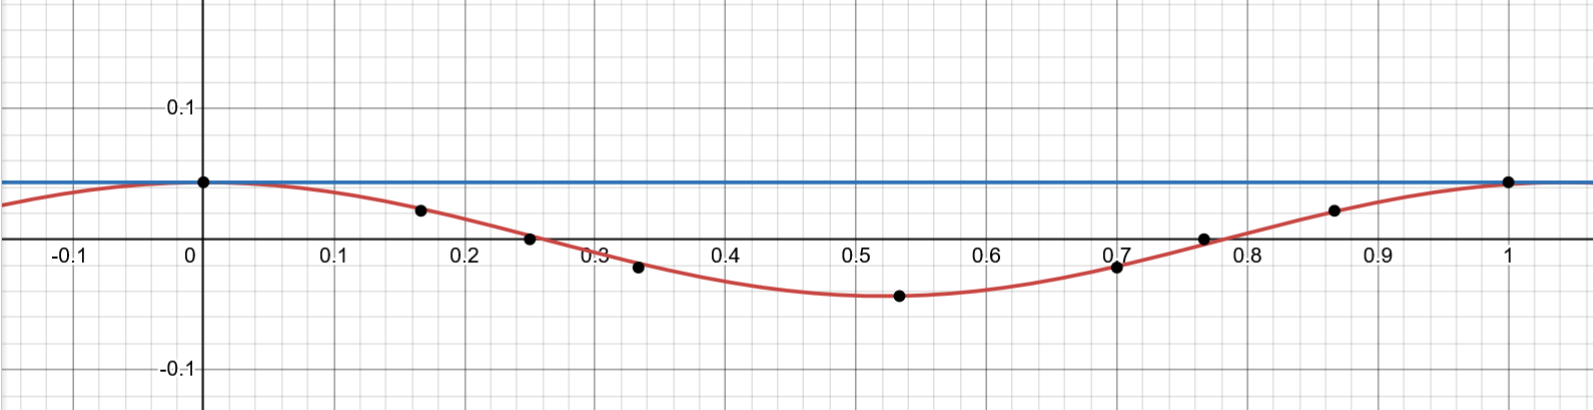
\includegraphics[width=0.74\textwidth]{Практ_2,5.png} \\ \hline
5^$\circ$   & 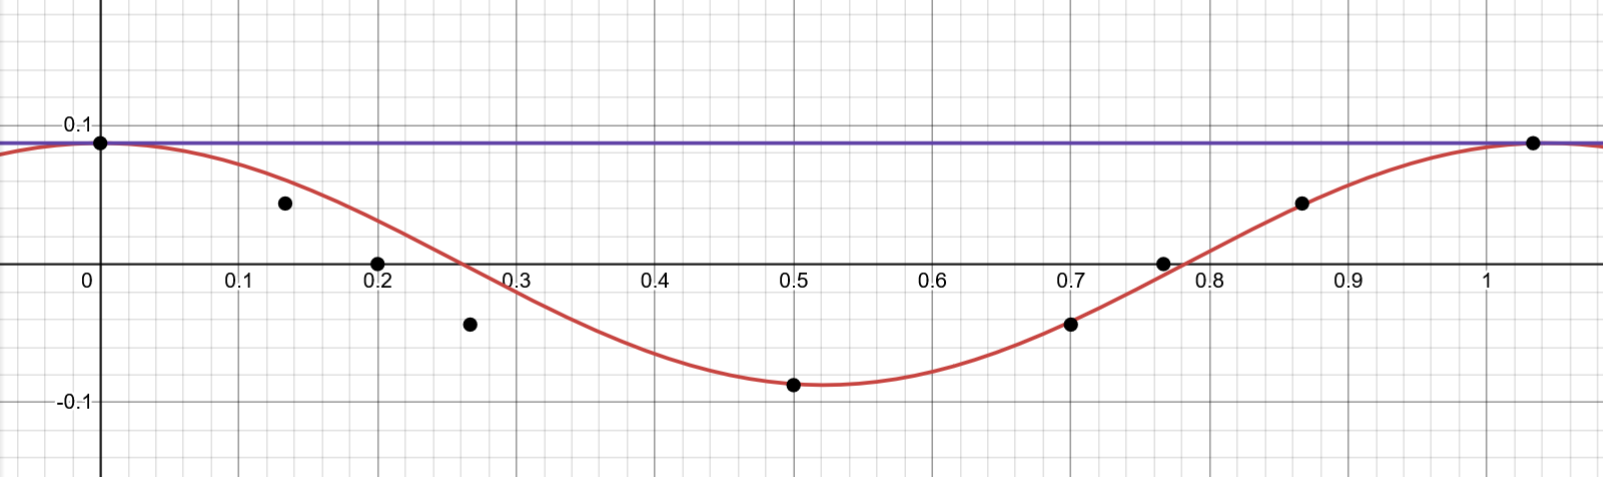
\includegraphics[width=0.74\textwidth]{Практ_5.png} \\ \hline
10$^\circ$  & 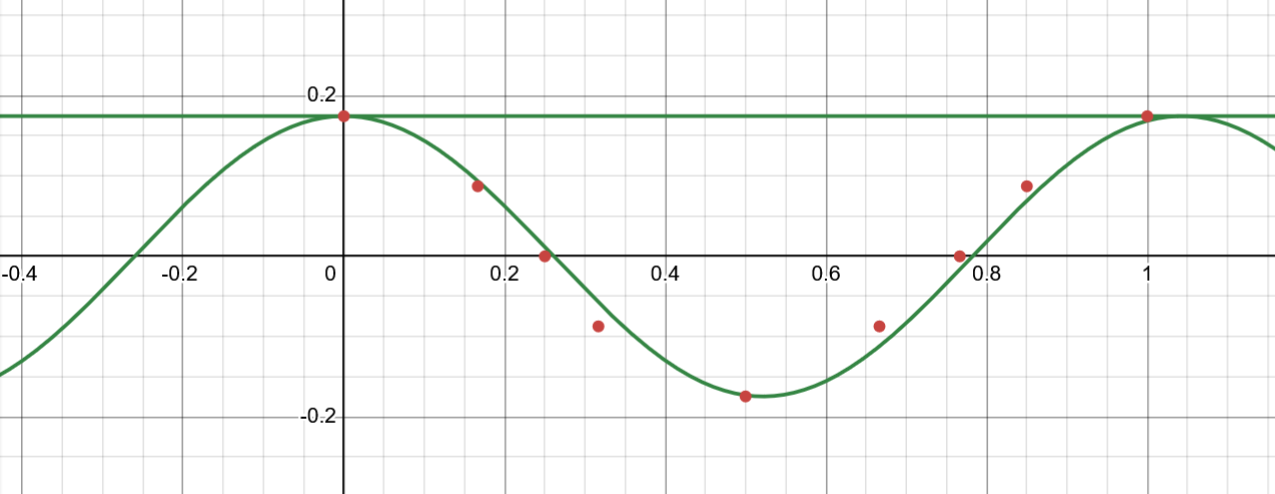
\includegraphics[width=0.75\textwidth]{Практ_10.png} \\ \hline
15$^\circ$  & 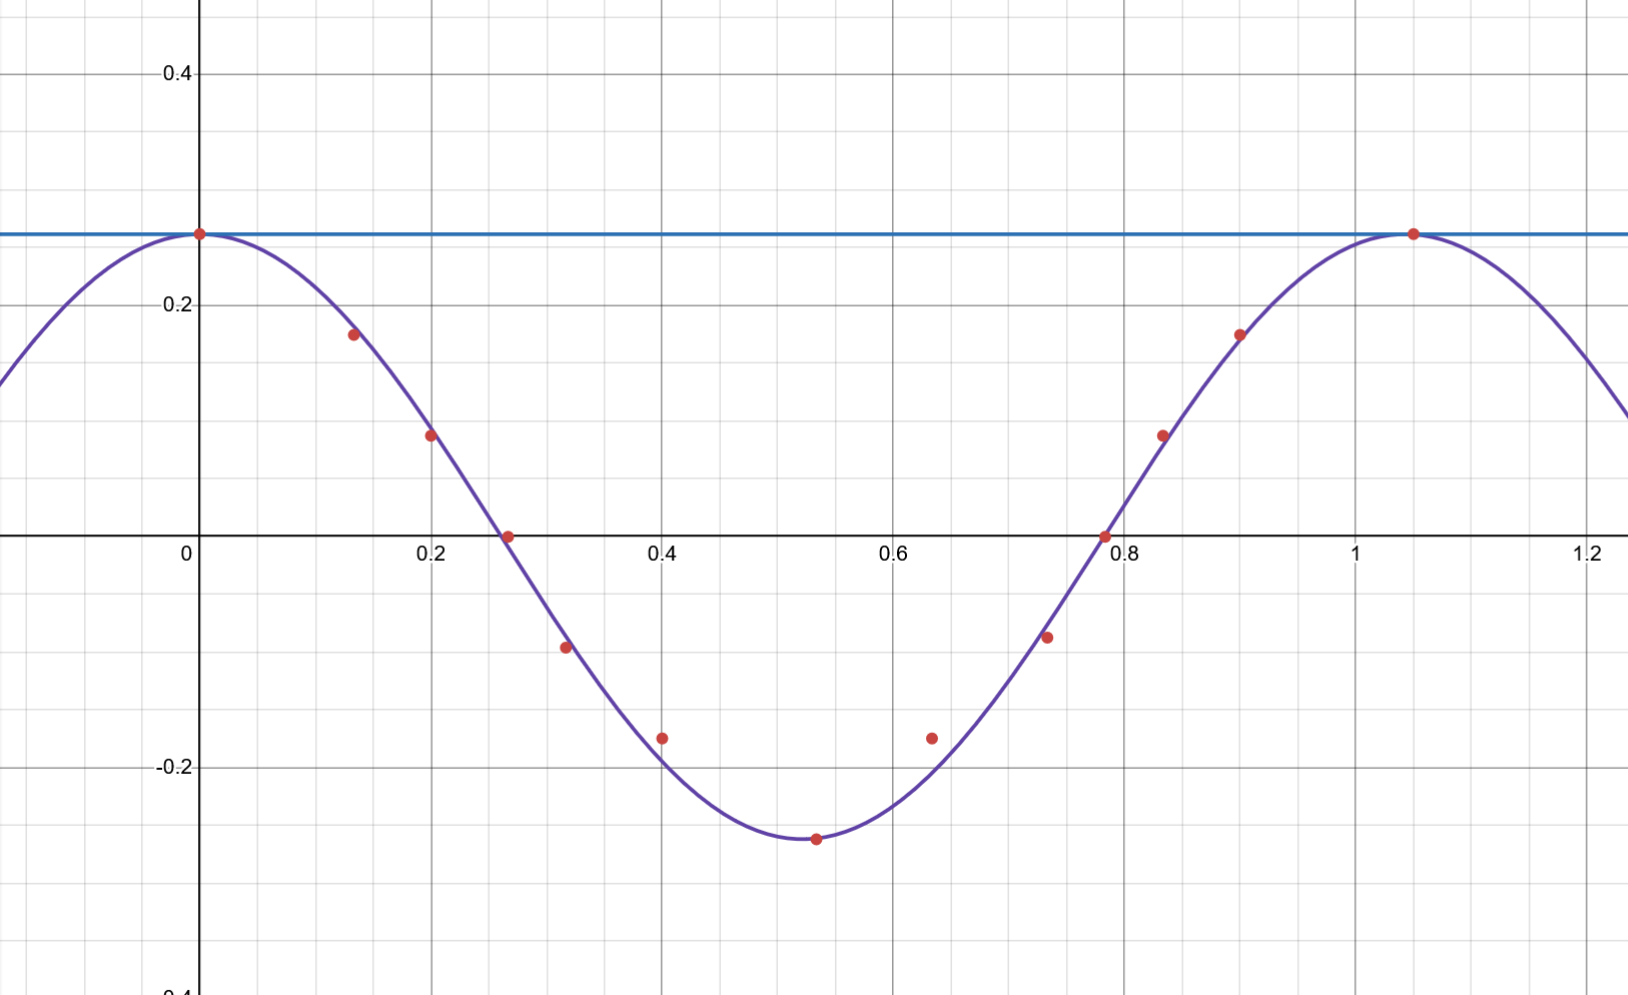
\includegraphics[width=0.74\textwidth]{Практ_15.png} \\ \hline
\end{tabular}

\vspace{0.5cm}
\\ Из графиков видно что точность в эксперименте достаточно высока.
\\ "линейность" зависимости лучше всего проявляется в окрестности 0, что видно из графиков: при углах от 2,5 до 15 погрешность минимальна.
\\ Видно, что при угле 15$^\circ$ погрешность меньше чем при 5$^\circ$. Это объясняется неидеальными условиями проведения эксперимента

\newpage
\subsection{Погрешности}
\subsubsection{ Причины погрешности в пунктах }эксперимента:
\\1.Приближение малых углов: Формула (4) получена из условия $\sin \theta \approx \theta$. При увеличении угла (особенно к 20°) эта ошибка растет, и реальный период становится больше теоретического.
\\2.Инструментальная погрешность: Ошибка при определении момента начала и конца колебания по видео или секундомеру.
\\3.Физические факторы: Сопротивление воздуха и трение в точке подвеса, которые не учитываются в уравнении 
\\4.Параметры установки: Погрешность измерения длины нити L от точки подвеса до центра масс груза.

\vspace{0.5cm}
\subsubsection{Объяснение перехода в (3)}
\\ Из конспекта становится ясно, что
переход в (3) объясняется тем, что после упрощения синуса до угла ($\sin \theta \approx \theta$) движение маятника становится гармоническим. Решением такого типа дифференциальных уравнений являются синусоидальные функции \cite{1}, а выбор косинуса продиктован начальным условием: в момент пуска маятник максимально отклонен, а его скорость равна нулю.($\sin(0) = 0$ (маятник начинал бы движение из центра), а косинус $\cos(0) = 1$)

\subsubsection{Рассчет погрешностей}
\[
\varepsilon = \frac{|T_{\text{практ}} - T_{\text{теор}}|}{T_{\text{теор}}} \cdot 100\% = \frac{\Delta T}{T}\cdot 100\%\]
\[
\varepsilon_1 = \frac{0.00354496158}{1.00354496158} \cdot 100\% \approx 0.35\% 
\]
\[
\varepsilon_2 = \frac{0.01645503842}{1.00354496158} \cdot 100\% \approx 1.64\% 
\]
\[
\varepsilon_3 = \frac{0.00354496158}{1.00354496158} \cdot 100\% \approx 0.35\% 
\]
\[
\varepsilon_3 = \frac{0,14645503842}{1,00354496158} \cdot 100\% \approx 14.59\% 
\]

\subsection{Вывод}
1.Экспериментально подтверждено, что для малых углов ($2{,}5^\circ$–$10^\circ$) линейная модель маятника описывает движение с высокой точностью (относительная погрешность $\varepsilon < 2\%$). Это доказывает справедливость допущения $\sin \theta \approx \theta$ в данном диапазоне.
\\ \\2.Зависимость периода от амплитуды: В ходе опыта выявлено, что при увеличении угла до $15^\circ$ погрешность существенно возрастает (до $14{,}59\%$), а практический период становится заметно больше теоретического. Это подтверждает, что при выходе за границы «малых углов» линейная формула начинает давать существенную ошибку.
\\ \\3.Анализ расхождений на графиках: Визуальный анализ графиков показывает, что экспериментальные точки в начале колебания практически идеально ложатся на теоретическую кривую, но со временем наблюдается фазовый сдвиг. Это свидетельствует о накоплении погрешности из-за разницы периодов модели и реальности.


\begin{thebibliography}{5}
\bibitem{1} 
Савельев И. В. «Курс общей физики» (Том 1).
 * Формулировка: «Согласно теории гармонических колебаний, общее решение уравнения $\theta^{\prime\prime} + \omega^2 \theta = 0$ имеет вид $\theta(t) = A \cos(\omega t + \alpha)$, где $A$ — амплитуда, а $\alpha$ — начальная фаза, определяемые из начальных условий».
\end{thebibliography}
